
\documentclass[tikz,border=6pt]{standalone}
\usepackage[T1]{fontenc}
\usepackage{mathpazo}
\usepackage{amsmath,amssymb,booktabs}
\usepackage{xcolor}
\usepackage{pagecolor}
\usepackage{pgfplots}
\usepackage{pgfplotstable}
\usepgfplotslibrary{groupplots}
\usepackage{tikz}
\usetikzlibrary{arrows.meta,backgrounds,calc,decorations.pathreplacing,fit,matrix,positioning,shapes.geometric}
\pgfplotsset{compat=1.18}
\definecolor{ink}{HTML}{1F2937}
\definecolor{teal}{HTML}{1D7874}
\definecolor{rust}{HTML}{C75C36}
\definecolor{gold}{HTML}{D9A441}
\definecolor{sage}{HTML}{6C9A8B}
\definecolor{berry}{HTML}{9E2A2B}
\definecolor{sand}{HTML}{F3E9D2}
\definecolor{mist}{HTML}{E7EEF3}
\definecolor{charcoal}{HTML}{3C4858}
\pagecolor{white}
\color{ink}
\pgfplotsset{paperaxis/.style={
    font=\small,
    tick label style={font=\small},
    label style={font=\small},
    title style={font=\small\bfseries},
    every axis plot/.append style={line width=1.2pt},
    grid=both,
    major grid style={draw=mist},
    minor grid style={draw=mist!60},
    grid style={line width=0.2pt},
    axis line style={draw=charcoal},
    tick style={draw=charcoal},
    legend style={draw=none, fill=white, font=\small, row sep=2pt, column sep=4pt}
}}

\begin{document}
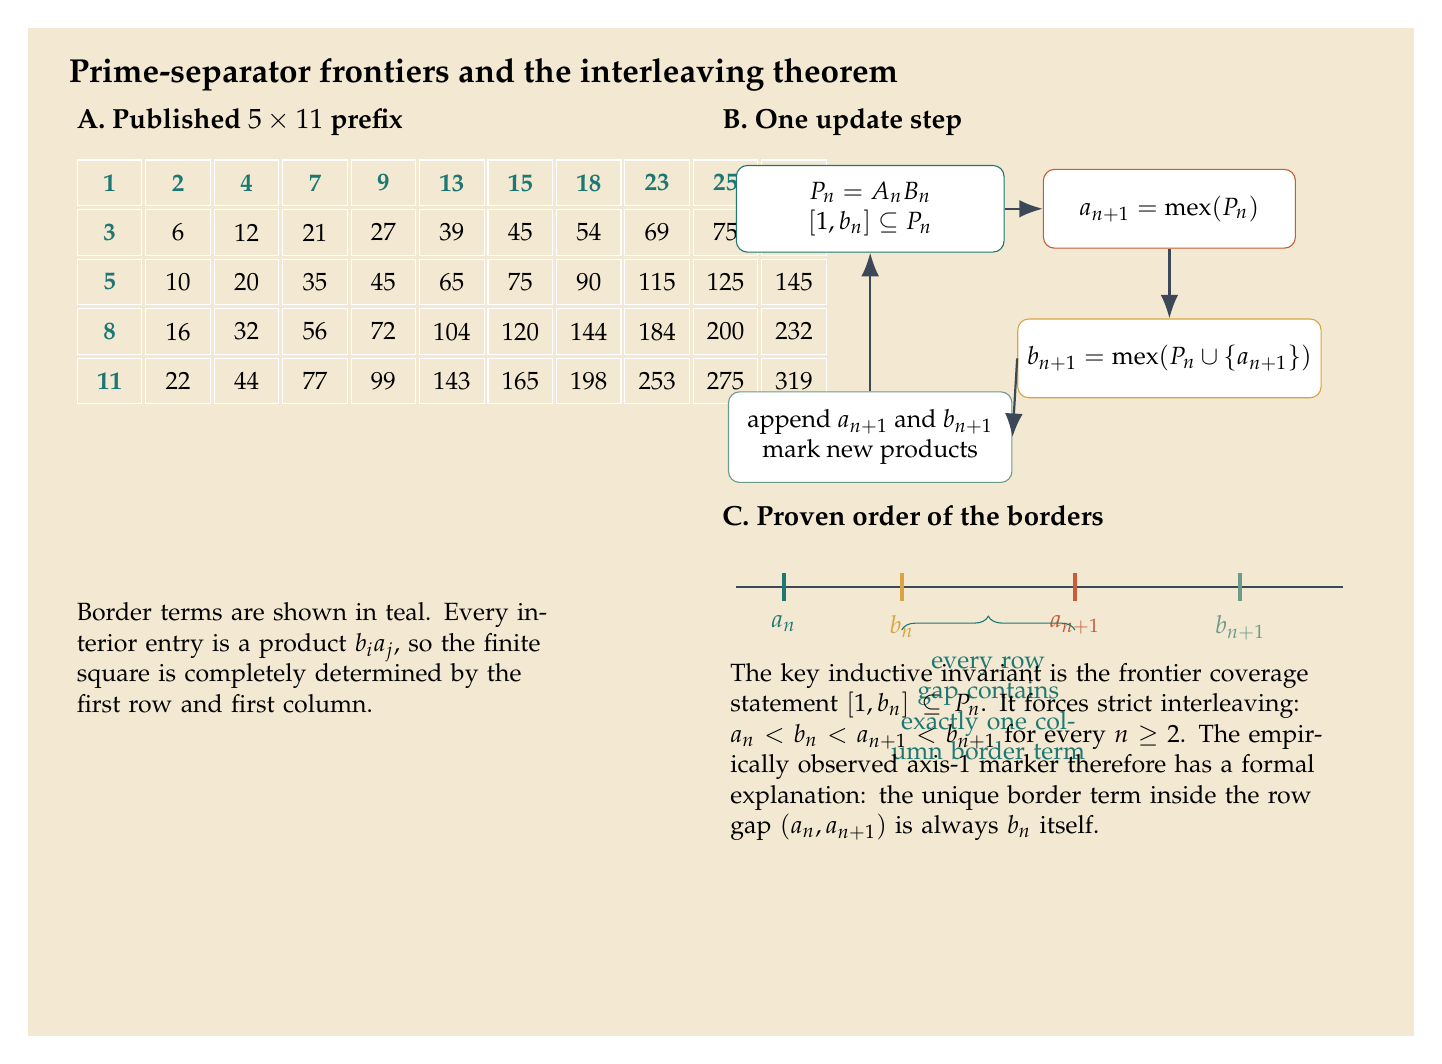
\begin{tikzpicture}[font=\small]
  \fill[sand] (-0.5,-6.7) rectangle (17.1,6.1);
  \node[anchor=west,font=\bfseries\large] at (-0.1,5.5) {Prime-separator frontiers and the interleaving theorem};

  \node[anchor=west,font=\bfseries] at (0.0,4.9) {A. Published $5\times 11$ prefix};
  \matrix[matrix of nodes,
          nodes={draw=white, minimum width=0.82cm, minimum height=0.58cm, anchor=center},
          column sep=1pt,row sep=1pt,
          nodes in empty cells,
          anchor=north west] (tbl) at (0.0,4.55) {
\textcolor{teal}{\bfseries 1} & \textcolor{teal}{\bfseries 2} & \textcolor{teal}{\bfseries 4} & \textcolor{teal}{\bfseries 7} & \textcolor{teal}{\bfseries 9} & \textcolor{teal}{\bfseries 13} & \textcolor{teal}{\bfseries 15} & \textcolor{teal}{\bfseries 18} & \textcolor{teal}{\bfseries 23} & \textcolor{teal}{\bfseries 25} & \textcolor{teal}{\bfseries 29} \\
\textcolor{teal}{\bfseries 3} & 6 & 12 & 21 & 27 & 39 & 45 & 54 & 69 & 75 & 87 \\
\textcolor{teal}{\bfseries 5} & 10 & 20 & 35 & 45 & 65 & 75 & 90 & 115 & 125 & 145 \\
\textcolor{teal}{\bfseries 8} & 16 & 32 & 56 & 72 & 104 & 120 & 144 & 184 & 200 & 232 \\
\textcolor{teal}{\bfseries 11} & 22 & 44 & 77 & 99 & 143 & 165 & 198 & 253 & 275 & 319 \\
  };
  \node[anchor=west, align=left, text width=6.2cm] at (0.0,-1.9) {
    Border terms are shown in teal. Every interior entry is a product $b_i a_j$, so the
    finite square is completely determined by the first row and first column.
  };

  \node[anchor=west,font=\bfseries] at (8.2,4.9) {B. One update step};
  \node[draw=teal, rounded corners=4pt, fill=white, minimum width=3.4cm, minimum height=1.1cm, align=center] (pn) at (10.2,3.8) {$P_n = A_n B_n$\\$[1,b_n]\subseteq P_n$};
  \node[draw=rust, rounded corners=4pt, fill=white, minimum width=3.2cm, minimum height=1.0cm, align=center] (an) at (14.0,3.8) {$a_{n+1}=\mathrm{mex}(P_n)$};
  \node[draw=gold, rounded corners=4pt, fill=white, minimum width=3.2cm, minimum height=1.0cm, align=center] (bn) at (14.0,1.9) {$b_{n+1}=\mathrm{mex}(P_n\cup\{a_{n+1}\})$};
  \node[draw=sage, rounded corners=4pt, fill=white, minimum width=3.6cm, minimum height=1.15cm, align=center] (upd) at (10.2,0.9) {append $a_{n+1}$ and $b_{n+1}$\\mark new products};
  \draw[-{Latex[length=3mm]}, thick, charcoal] (pn.east) -- (an.west);
  \draw[-{Latex[length=3mm]}, thick, charcoal] (an.south) -- (bn.north);
  \draw[-{Latex[length=3mm]}, thick, charcoal] (bn.west) -- (upd.east);
  \draw[-{Latex[length=3mm]}, thick, charcoal] (upd.north) -- ++(0,0.75) -| (pn.south);

  \node[anchor=west,font=\bfseries] at (8.2,-0.1) {C. Proven order of the borders};
  \draw[charcoal, line width=0.8pt] (8.5,-1.0) -- (16.2,-1.0);
  \foreach \x/\lab/\col in {9.1/{$a_n$}/teal, 10.6/{$b_n$}/gold, 12.8/{$a_{n+1}$}/rust, 14.9/{$b_{n+1}$}/sage} {
    \draw[\col, line width=1.4pt] (\x,-0.82) -- (\x,-1.18);
    \node[anchor=north, text=\col] at (\x,-1.24) {\lab};
  }
  \draw[decorate, decoration={brace, amplitude=5pt}, teal] (10.6,-1.55) -- node[below=6pt, align=center, text width=3.0cm] {every row gap contains\\exactly one column border term} (12.8,-1.55);

  \node[anchor=west, align=left, text width=7.7cm] at (8.3,-3.1) {
    The key inductive invariant is the frontier coverage statement $[1,b_n]\subseteq P_n$.
    It forces strict interleaving:
    $a_n < b_n < a_{n+1} < b_{n+1}$ for every $n\ge 2$.
    The empirically observed axis-1 marker therefore has a formal explanation:
    the unique border term inside the row gap $(a_n,a_{n+1})$ is always $b_n$ itself.
  };
\end{tikzpicture}
\end{document}
